% === T02 - Memoria Dinámica ===
% David Alejandro Gonzalez Marquez
% fokerman@gmail.com
% https://github.com/fokerman/computingSystemsCourse

\documentclass[aspectratio=169]{beamer}
\usepackage{../packages}

\usepackage{listings}

\title{\Huge Memoria Dinámica}
\author{David Alejandro González Márquez}
\input{../university}
\date{}

\begin{document}

\begin{frame}[plain]
    \titlepage
    \begin{textblock}{100}(30,80)
    \begin{tcolorbox}[size=small,width=\textwidth,colback={gray!30},title={}]
    \begin{center}
     \scriptsize Clase disponible en: \url{https://github.com/fokerman/computingSystemsCourse}
    \end{center}
    \end{tcolorbox}
    \end{textblock}
%     \begin{textblock}{140}(10,70)
%     \textcolor{rojo}{
%     \textbf{Atención}: La clase será grabada por el anfitrión para su posterior y eventual uso académico dentro de nuestra institución. Su participación en la clase implica brindar su consentimiento para participar en la grabación, aunque pueden mantener su video apagado.}
%     \end{textblock}
\end{frame}

\begin{frame}[fragile,t]{Memoria}
    \begin{textblock}{87}(10,10)
    \only<2->{
    \begin{block}{Variable estática}
    Asignada en un espacio de memoria \textbf{reservado} que solo será utilizado para almacenar la variable en cuestión.
    \end{block}
    }
    \end{textblock}
    \begin{textblock}{87}(10,30)
    \only<3->{
    \begin{block}{Variable en la pila}
    Esta asignada dentro del espacio de \textbf{pila} del programa, puede existir solo en el contexto de ejecución de una función.
    \end{block}
    }
    \end{textblock}
    \begin{textblock}{87}(10,55)
    \only<4->{
    \begin{block}{Variable dinámica}
    Esta asignada en un espacio de memoria \textbf{solicitado al sistema} operativo mediante una biblioteca de funciones, estas permiten solicitar y liberar memoria. (\texttt{malloc})
    \end{block}
    }
    \end{textblock}
    \begin{textblock}{100}(100,7)
    \small
    \only<2->{
    \textcolor{gray}{Ejemplo:}\\
    \texttt{\#include <stdio.h>}\\
    \texttt{...}\\
    \textcolor{red}{\texttt{int numero = 10;}}\\
    \textcolor{red}{\texttt{const char* letra = "10"}}\\ % \textquotesingle{}
    \texttt{...}\\
    }
    \only<3->{
    \texttt{int main() \{}\\
    \hspace{0.8cm} \texttt{...}\\
    \hspace{0.8cm} \textcolor{red}{\texttt{int n = 10;}}\\
    \hspace{0.8cm} \textcolor{red}{\texttt{int* puntero;}}\\
    \hspace{0.8cm} \texttt{...}\\
    }
    \only<4->{
    \hspace{0.8cm} \texttt{...}\\
    \hspace{0.8cm} \texttt{...}\\
    \hspace{0.8cm} \textcolor{red}{\texttt{int* puntero = malloc(10);}}\\
    \hspace{0.8cm} \texttt{...}\\
    \hspace{0.8cm} \textcolor{red}{\texttt{free(puntero);}}\\
    \hspace{0.8cm} \texttt{...}\\
    \texttt{\}}\\
    }
    \end{textblock}
\end{frame}

\begin{frame}{Memoria}
    \begin{textblock}{100}(7,14) \only<1->{\includegraphics[scale=0.9]{img/memory-layer1.pdf}} \end{textblock} % direcciones altas bajas
    \begin{textblock}{100}(7,14) \only<2->{\includegraphics[scale=0.9]{img/memory-layer2.pdf}} \end{textblock} % segmento data text (TEXTO) 
    \begin{textblock}{100}(7,14) \only<2->{\includegraphics[scale=0.9]{img/memory-layer3.pdf}} \end{textblock} % segmento data text
    \begin{textblock}{100}(7,14) \only<3->{\includegraphics[scale=0.9]{img/memory-layer4.pdf}} \end{textblock} % segmento bss stack (TEXTO)
    \begin{textblock}{100}(7,14) \only<3->{\includegraphics[scale=0.9]{img/memory-layer5.pdf}} \end{textblock} % segmento bss stack
    \begin{textblock}{100}(7,14) \only<4->{\includegraphics[scale=0.9]{img/memory-layer6.pdf}} \end{textblock} % segmento heap (TEXTO) 
    \begin{textblock}{100}(7,14) \only<4->{\includegraphics[scale=0.9]{img/memory-layer7.pdf}} \end{textblock} % segmento heap
\end{frame}

\begin{frame}{Memoria}
    \begin{textblock}{100}(7,14) \only<1->{\includegraphics[scale=0.9]{img/memory-layer1.pdf}} \end{textblock} % direcciones altas bajas
    \begin{textblock}{100}(7,14) \only<1->{\includegraphics[scale=0.9]{img/memory-layer3.pdf}} \end{textblock} % segmento data text
    \begin{textblock}{100}(7,14) \only<1->{\includegraphics[scale=0.9]{img/memory-layer5.pdf}} \end{textblock} % segmento bss stack
    \begin{textblock}{100}(7,14) \only<1->{\includegraphics[scale=0.9]{img/memory-layer7.pdf}} \end{textblock} % segmento heap
    \begin{textblock}{100}(7,14) \only<2->{\includegraphics[scale=0.9]{img/memory-layer8.pdf}} \end{textblock} % text
    \begin{textblock}{100}(7,14) \only<3->{\includegraphics[scale=0.9]{img/memory-layer9.pdf}} \end{textblock} % data
    \begin{textblock}{100}(7,14) \only<4->{\includegraphics[scale=0.9]{img/memory-layer10.pdf}} \end{textblock} % bss
    \begin{textblock}{100}(7,14) \only<5->{\includegraphics[scale=0.9]{img/memory-layer11.pdf}} \end{textblock} % stack
    \begin{textblock}{100}(7,14) \only<6->{\includegraphics[scale=0.9]{img/memory-layer12.pdf}} \end{textblock} % heap
    \begin{textblock}{100}(7,14) \only<1->{\includegraphics[scale=0.9]{img/memory-layer13.pdf}} \end{textblock} % codigo
\end{frame}

\begin{frame}[t]{Memoria Dinámica}
    \begin{block}{Solicitar memoria}
    \begin{center}
    \textcolor{verdeuca}{\texttt{void *malloc(size\_t size)}}\\
    \end{center}
    Asigna \texttt{size} bytes de memoria y nos devuelve su posición.
    \end{block}
    \vspace{0.5cm}
    \pause
    \begin{block}{Liberar memoria}
    \begin{center}
    \textcolor{verdeuca}{\texttt{void free(void *pointer)}}\\
    \end{center}
    Libera la memoria en \texttt{pointer}, previamente solicitada por \texttt{malloc}.
    \end{block}
    \pause
    \vspace{0.3cm}
    \begin{center}
    \textit{``With a great power comes a great responsibility''} 
    \end{center}
\end{frame}

\begin{frame}[fragile,t]{Memoria Dinámica  \hspace{0.5cm}\huge - IMPORTANTE -}
    \normalsize
    Si se solicita memoria utilizando \texttt{malloc}, se \textbf{DEBE} liberar utilizando \texttt{free}.\\
    Toda memoria que se solicite \textbf{DEBE} ser liberada durante la ejecución del programa.\\
    \vspace{0.3cm}
    \pause
    Caso contrario se \hspace{0.03cm} \huge \textcolor{red}{PIERDE MEMORIA} \\
    \vspace{0.3cm}
    \pause
    \normalsize Para detectar problemas en el uso de la memoria se puede utilizar: \\
    \begin{center}
    \Huge \texttt{Valgrind}\\
    \end{center}
    \pause
    \normalsize \textcolor{verdeuca}{Uso:}\\
    \normalsize \verb|$ valgrind --leak-check=full --show-leak-kinds=all -v ./holamundo|\\
    \vspace{0.2cm}
    \normalsize \textcolor{verdeuca}{Instalación:}\\
    \begin{itemize}
    \item[-] Ubuntu/Debian: \texttt{sudo apt-get install valgrind}
    \item[-] Otros Linux: \url{http://valgrind.org/downloads/current.html}
    \item[-] Windows/Mac OS: \textcolor{naranjauca}{usen Linux}
    \end{itemize}
\end{frame}

% \begin{frame}{Repaso de punteros}
%     \begin{itemize}
%     \setlength\itemsep{1.2em}
%     \item Es una variable que referencia una \textbf{posición de la memoria}.\\ \small (ejemplo: una variable cuyo valor es una dirección de memoria) \normalsize
%     \pause
%     \item Tiene un tipo y un nombre.
%     \pause
%     \item Almacena una dirección de memoria.
%     \pause
%     \item Sirve para referenciar una posición de memoria.
%     \pause
%     \item Operadores:
%     \begin{itemize}
%     \pause
%     \item[\textbf{\&}] $\rightarrow$ Da como resultado la dirección de memoria de una variable.
%     \pause
%     \item[\textbf{*}] $\rightarrow$ Da como resultado el valor apuntado por un puntero.\\ \hskip 0.5cm \footnotesize (Además de ser el indicador del tipo puntero)\normalsize
%     \end{itemize}
%     \end{itemize}
% \end{frame}

% \begin{frame}[fragile]{Repaso de punteros}
%     \framesubtitle{Ejemplos:}
%     \begin{itemize}
%     \item \verb|int *pepe| \\ \vskip 0.1cm
%     \pause
%     Declara un puntero de tipo entero con nombre \textit{pepe}.
%     \vskip 0.3cm
%     \pause
%     \item \verb|int x = 5|\\
%     \verb|pepe = &x|\\ \vskip 0.1cm
%     \pause
%     Guarda en el puntero \textit{pepe} la dirección de \textit{x}. Se dice que \textit{pepe} apunta a \textit{x}.\\
%     \vskip 0.3cm
%     \pause
%     \item \verb|*pepe = 8|\\ \vskip 0.1cm
%     \pause
%     Guarda 8 en la posición apuntada por el puntero \textit{pepe}.
%     \vskip 0.3cm
%     \pause
%     \item \verb|int y|\\
%     \verb|y = *pepe|\\ \vskip 0.1cm
%     Guarda en \textit{y} el valor apuntado por \textit{pepe}.
%     \end{itemize}
% \end{frame}

% \begin{frame}[fragile]{Repaso de punteros}
%     \framesubtitle{Ejemplos:}
%     \begin{textblock}{50}(10,15)
%     \begin{enumerate}
%     \setlength\itemsep{1.5em}
%     \Large
%     \item \verb|int *pepe|
%     \vskip 0.3cm
%     \item \verb|int x = 5|\\
%     \verb|pepe = &x|
%     \vskip 0.3cm
%     \item \verb|*pepe = 8|
%     \vskip 0.3cm
%     \item \verb|int y|\\
%     \verb|y = *pepe|
%     \vskip 0.3cm
%     \end{enumerate}
%     \end{textblock}
%     \begin{textblock}{50}(90,15)
%     \only<1>{\Large 1.}
%     \only<2>{\Large 2.}
%     \only<3>{\Large 3.}
%     \only<4>{\Large 4.}
%     \end{textblock}
%     \begin{textblock}{50}(90,20) \only<1->{\includegraphics[scale=1]{img/punteros-layer1.pdf}} \end{textblock}
%     \begin{textblock}{50}(90,20) \only<2->{\includegraphics[scale=1]{img/punteros-layer2.pdf}} \end{textblock}
%     \begin{textblock}{50}(90,20) \only<3->{\includegraphics[scale=1]{img/punteros-layer3.pdf}} \end{textblock}
%     \begin{textblock}{50}(90,20) \only<4->{\includegraphics[scale=1]{img/punteros-layer4.pdf}} \end{textblock}
% \end{frame}

\begin{frame}[fragile]{Arreglos}
    \begin{beamercolorbox}[wd=1\textwidth,sep=1em]{coloredboxstuffNaranja}
    \centering \large
    Un arreglo o vector es una secuencia ordenada de elementos\\ consecutivos en memoria de un tamaño fijo.
    \end{beamercolorbox}
    \bigskip
    \begin{center}
    \large
    \begin{tabular}{|C{0.8cm}|C{0.8cm}|C{0.8cm}|C{1.8cm}|C{0.8cm}|C{0.8cm}|C{0.8cm}|}
     \hline
     $A_0$ & $A_1$ & $A_2$ & $\cdots$ & $A_{n-3}$ & $A_{n-2}$ & $A_{n-1}$ \\
     \hline
    \end{tabular}
    \end{center}
\end{frame}

\begin{frame}[fragile]{Arreglos}
    Declaremos un vector \textit{v} en \texttt{C}:\\
    \bigskip
    \pause
    \begin{beamercolorbox}[wd=0.9\textwidth,sep=0.5em]{coloredboxstuffVerde}
    \verb|int v[5];|
    \end{beamercolorbox}
    \bigskip
    ¿Cómo está guardado en memoria?\\
    \bigskip
    \pause
    Como 5 enteros (\textit{doublewords} / 4 bytes) \textbf{consecutivos:}\\
    \bigskip
    \begin{center}
    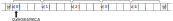
\includegraphics[scale=0.8]{img/vector.pdf}
    \end{center}
\end{frame}

% \begin{frame}[fragile]{Arreglos}
%     Si rememoramos el ejemplo del hola mundo en ASM:\\
%     \bigskip
%     \begin{beamercolorbox}[wd=0.9\textwidth,sep=0.5em]{coloredboxstuffVerde}
%     \verb|section .rodata:|\\
%     \verb|msg: DB 'Hola mundo', 10, 0|\\
%     \verb|largo: EQU $-msg-1|
%     \end{beamercolorbox}
%     \bigskip
%     \pause
%     \texttt{msg} es una etiqueta que, vista como un puntero,\\ es un vector de caracteres almacenados de la siguiente manera:
%     
%     \begin{center}
%     \includegraphics[scale=0.6,keepaspectratio]{img/holamundo.pdf}
%     \end{center}
%     \pause
%     \small \texttt{msg} es un \texttt{char*}, es como si en \texttt{C} hiciéramos:\\
%     \small
%     \begin{beamercolorbox}[wd=0.9\textwidth,sep=0.5em]{coloredboxstuffVerde}
%     \verb|char msg[11] = "Hola mundo\n";|
%     \end{beamercolorbox}
% \end{frame}

\begin{frame}[fragile,t]{Arreglos}
    Dado:\\
    \vskip 5pt
    \begin{beamercolorbox}[wd=0.9\textwidth,sep=0.5em]{coloredboxstuffVerde}
    \verb|int v[5];|\\
    \end{beamercolorbox}
    \pause
    Si suponemos que el primer elemento se encuentra almacenado\\  en la dirección 0x200 de memoria\\
    \pause
    \vskip 5pt
    ¿cómo se realiza la siguiente asignación?
    \vskip 5pt
    \begin{beamercolorbox}[wd=0.9\textwidth,sep=0.5em]{coloredboxstuffVerde}
    \verb|v[2] = 8;|
    \pause
    \end{beamercolorbox}
    \begin{textblock}{50}(10,59) \only<4->{\includegraphics[scale=0.8]{img/vectorAnimado-layer1.pdf}} \end{textblock}
    \begin{textblock}{50}(10,59) \only<5->{\includegraphics[scale=0.8]{img/vectorAnimado-layer2.pdf}} \end{textblock}
    \begin{textblock}{50}(10,59) \only<6->{\includegraphics[scale=0.8]{img/vectorAnimado-layer3.pdf}} \end{textblock}
    \begin{textblock}{50}(10,59) \only<7->{\includegraphics[scale=0.8]{img/vectorAnimado-layer4.pdf}} \end{textblock}
    \begin{textblock}{50}(10,59) \only<8->{\includegraphics[scale=0.8]{img/vectorAnimado-layer5.pdf}} \end{textblock}
\end{frame}

\begin{frame}[fragile]{Arreglos y Punteros}
    Si tenemos:
    \vskip 5pt
    \begin{beamercolorbox}[wd=1\textwidth,sep=0.5em]{coloredboxstuffVerde}
    \verb|int v[5];| 
    \end{beamercolorbox}
    \vskip 5pt
    \textit{v} es un puntero al primer elemento del vector.\\ 
    \vskip 15pt
    \pause
    Luego, vale en \texttt{C}:
    \vskip 15pt
    \begin{beamercolorbox}[wd=1\textwidth,sep=0.5em]{coloredboxstuffVerde}
    \verb| int *p = v;| $\leftarrow$ \footnotesize tomo el puntero al vector
    \end{beamercolorbox}
    \begin{center}
    \vskip -7pt
    ó
    \end{center}
    \begin{beamercolorbox}[wd=1\textwidth,sep=0.5em]{coloredboxstuffVerde}
    \verb| int *p = &(v[0]);| $\leftarrow$ \footnotesize tomo la dirección del primer elemento
    \end{beamercolorbox}
\end{frame}

\begin{frame}[fragile]{Arreglos}
    ¿Cómo solicitar memoria dinámica para un vector de 100 enteros de 32 bits?\\
    \bigskip
    \pause
    \begin{beamercolorbox}[wd=0.9\textwidth,sep=0.5em]{coloredboxstuffVerde}
    \verb|int* v = (int*) malloc( sizeof(int) * 100 );|
    \end{beamercolorbox}
    \pause
    \bigskip
    \textbf{\texttt{sizeof} es un operador de C} que dado un nombre de un tipo de datos\\
    retorna la cantidad de bytes que ocupa. En este caso 4 bytes.\\
    \bigskip
    La operación \textbf{\texttt{(int*)}} delante de \texttt{malloc} indica a C que el resultado de la función\\
    debe ser considerado como un puntero a entero. Esta operación se denomina \texttt{casting}.\\
    \bigskip
    \begin{center}
    \textcolor{verdeuca}{
    En este caso el resultado de \emph{malloc} será un puntero a un área de\\ memoria de 400 bytes donde caben 100 enteros de 32 bits.
    }
    \end{center}
\end{frame}

\begin{frame}[fragile]{Ejemplo de Arreglos}
    \begin{textblock}{65}(8,15) \small 
    \uncover<3->{Considerar un arreglo que representa una barra lineal, con un extremo a 200\textcelsius\xspace y otro a 25\textcelsius\xspace.\\}
    \medskip
    \uncover<4->{Inicialmente se \textbf{solicita memoria} y se inicializa en cero todo el arreglo.\\}
    \medskip
    \uncover<5->{Luego se completan las \textbf{condiciones iniciales} de temperatura en ambos extremos.\\}
    \medskip
    \uncover<6->{Por último, el sistema \textbf{evoluciona en cada interación} calculando para cada celda el promedio de las celdas contiguas.\\}
    \end{textblock}
    \begin{textblock}{50}(5,70) \only<2->{\includegraphics[scale=1]{img/ejemploDifusion-layer1.pdf}} \end{textblock}
    \begin{textblock}{50}(5,70) \only<3->{\includegraphics[scale=1]{img/ejemploDifusion-layer2.pdf}} \end{textblock}
    \begin{textblock}{50}(5,70) \only<4->{\includegraphics[scale=1]{img/ejemploDifusion-layer3.pdf}} \end{textblock}
    \begin{textblock}{50}(5,70) \only<5->{\includegraphics[scale=1]{img/ejemploDifusion-layer4.pdf}} \end{textblock}
    \begin{textblock}{50}(5,70) \only<6->{\includegraphics[scale=1]{img/ejemploDifusion-layer5.pdf}} \end{textblock}
    \begin{textblock}{50}(5,70) \only<7->{\includegraphics[scale=1]{img/ejemploDifusion-layer6.pdf}} \end{textblock}
    \begin{textblock}{50}(5,70) \only<8->{\includegraphics[scale=1]{img/ejemploDifusion-layer7.pdf}} \end{textblock}
    \begin{textblock}{50}(5,70) \only<9->{\includegraphics[scale=1]{img/ejemploDifusion-layer8.pdf}} \end{textblock}
    \begin{textblock}{50}(5,70) \only<10->{\includegraphics[scale=1]{img/ejemploDifusion-layer9.pdf}} \end{textblock}
    \begin{textblock}{50}(5,70) \only<11->{\includegraphics[scale=1]{img/ejemploDifusion-layer10.pdf}} \end{textblock}

    \begin{textblock}{100}(80,2)
    \scriptsize
    \begin{lstlisting}[language=C,basicstyle=\ttfamily,columns=fullflexible]
void diffusionStep(float* data, int size) {
    for(int i=1; i<size-1; i++) {
        data[i] = (data[i-1]+data[i]+data[i+1])/3.0;
    }
}

int main() {

    int size = 10;
    float* data = (float*)malloc(sizeof(float)*size);
    initZero(data,size);
    
    data[0] = 200.0;
    data[size-1] = 25.0;

    for(int step=0;step<300;step++) {
        diffusionStep(data, size);
        print(data,size);
    }

    free(data);

    return 0;
}
    \end{lstlisting}
    \end{textblock}
\end{frame}

\begin{frame}[t]
    \frametitle{Listas}
    \begin{textblock}{65}(10,15)
    Es una estructura de datos que consiste en nodos \textbf{enlazados} mediante punteros.\\
    \bigskip
    Cada nodo contiene datos y un \textbf{puntero al siguiente} nodo.\\
    \bigskip
    Los datos pueden ser tipos básicos o punteros a \textbf{cualquier tipo} de datos.\\
    \bigskip
    Una lista termina cuando su último nodo apunta a \textbf{null}.\\
    \bigskip
    Incluso puede ser \textbf{doblemente enlazada}, conteniendo en cada nodo, un puntero anterior.\\
    \end{textblock}
    \begin{textblock}{60}(80,5) \only<1->{\includegraphics[scale=0.55]{img/lista-layer1.pdf}} \end{textblock}
    \begin{textblock}{60}(80,20) \only<2->{\includegraphics[scale=0.55]{img/lista-layer2.pdf}} \end{textblock}
    \begin{textblock}{60}(80,40) \only<3->{\includegraphics[scale=0.55]{img/lista-layer3.pdf}} \end{textblock}
    \begin{textblock}{60}(80,65) \only<4->{\includegraphics[scale=0.55]{img/lista-layer4.pdf}} \end{textblock}
\end{frame}

\begin{frame}[t]
    \frametitle{Listas}
    Estructuras:
    \begin{multicols}{2}
    \begin{tabular}{l}
    \texttt{struct lista \{}      \\
    \texttt{      struct nodo *primero;} \\
    \texttt{\};}                  \\
    \hspace{4cm}
    \end{tabular}
    \columnbreak
    \begin{tabular}{lll}
    \texttt{struct nodo \{}     \\
    \texttt{      int dato;}    \\
    \texttt{      struct nodo *prox;}  \\
    \texttt{\};}                \\
    \end{tabular}
    \end{multicols}
    \begin{textblock}{100}(30,40) \only<2->{\includegraphics[scale=0.7]{img/lista_enteros-layer1.pdf}} \end{textblock}
    \begin{textblock}{100}(30,40) \only<3->{\includegraphics[scale=0.7]{img/lista_enteros-layer2.pdf}} \end{textblock}
    \begin{textblock}{100}(30,40) \only<4->{\includegraphics[scale=0.7]{img/lista_enteros-layer3.pdf}} \end{textblock}
    \begin{textblock}{100}(30,40) \only<5->{\includegraphics[scale=0.7]{img/lista_enteros-layer4.pdf}} \end{textblock}
    \begin{textblock}{100}(30,40) \only<6->{\includegraphics[scale=0.7]{img/lista_enteros-layer5.pdf}} \end{textblock}
\end{frame}

\begin{frame}[t]
    \frametitle{Listas - Agregar}
    \begin{textblock}{100}(20,5) \only<3->{\includegraphics[scale=0.7]{img/lista_enteros_agregar-layer9.pdf}} \end{textblock}  % p. nuevo
    \begin{textblock}{100}(20,5) \only<4->{\includegraphics[scale=0.7]{img/lista_enteros_agregar-layer7.pdf}} \end{textblock}  % dato
    \begin{textblock}{100}(20,5) \only<5->{\includegraphics[scale=0.7]{img/lista_enteros_agregar-layer11.pdf}} \end{textblock} % p. copia
    \begin{textblock}{100}(20,5) \only<1->{\includegraphics[scale=0.7]{img/lista_enteros_agregar-layer1.pdf}} \end{textblock}  % list
    \begin{textblock}{100}(20,5) \only<1-2>{\includegraphics[scale=0.7]{img/lista_enteros_agregar-layer2.pdf}} \end{textblock}  % arrow
    \begin{textblock}{100}(20,5) \only<2,6>{\includegraphics[scale=0.7]{img/lista_enteros_agregar-layer3.pdf}} \end{textblock}  % malloc flecha
    \begin{textblock}{100}(20,5) \only<2->{\includegraphics[scale=0.7]{img/lista_enteros_agregar-layer4.pdf}} \end{textblock}  % malloc
    \begin{textblock}{100}(20,5) \only<3->{\includegraphics[scale=0.7]{img/lista_enteros_agregar-layer5.pdf}} \end{textblock}  % next nuevo
    \begin{textblock}{100}(20,5) \only<3->{\includegraphics[scale=0.7]{img/lista_enteros_agregar-layer10.pdf}} \end{textblock} % p. nuevo
    \begin{textblock}{100}(20,5) \only<4->{\includegraphics[scale=0.7]{img/lista_enteros_agregar-layer8.pdf}} \end{textblock}  % dato gris
    \begin{textblock}{100}(20,5) \only<5->{\includegraphics[scale=0.7]{img/lista_enteros_agregar-layer12.pdf}} \end{textblock} % p. copia
    \begin{textblock}{100}(20,5) \only<5->{\includegraphics[scale=0.7]{img/lista_enteros_agregar-layer6.pdf}} \end{textblock}  % next 
     \begin{textblock}{100}(20,5) \only<6>{\includegraphics[scale=0.7]{img/lista_enteros_agregar-layer13.pdf}} \end{textblock} % ABC
     
    \begin{textblock}{100}(10,68)
    \begin{enumerate}[A]
    \item Crear el nuevo nodo usando \texttt{malloc} y asignar su contenido
    \item Conectar el nuevo nodo a su siguiente en la lista
    \item Conectar el puntero anterior en la lista al nuevo nodo
    \end{enumerate}
    \end{textblock}
\end{frame}

\begin{frame}[t]
    \frametitle{Listas - Borrar}
    \begin{textblock}{100}(40,5) \only<2->{\includegraphics[scale=0.7]{img/lista_enteros_borrar-layer5.pdf}} \end{textblock}  % amarillo
    \begin{textblock}{100}(40,5) \only<1->{\includegraphics[scale=0.7]{img/lista_enteros_borrar-layer1.pdf}} \end{textblock}  % list
    \begin{textblock}{100}(40,5) \only<1-2>{\includegraphics[scale=0.7]{img/lista_enteros_borrar-layer2.pdf}} \end{textblock}  % arrow original
    \begin{textblock}{100}(40,5) \only<4->{\includegraphics[scale=0.7]{img/lista_enteros_borrar-layer3.pdf}} \end{textblock}  % free
    \begin{textblock}{100}(40,5) \only<3->{\includegraphics[scale=0.7]{img/lista_enteros_borrar-layer4.pdf}} \end{textblock}  % blanco
    \begin{textblock}{100}(40,5) \only<3->{\includegraphics[scale=0.7]{img/lista_enteros_borrar-layer7.pdf}} \end{textblock}  % arrow
    \begin{textblock}{100}(40,5) \only<2->{\includegraphics[scale=0.7]{img/lista_enteros_borrar-layer6.pdf}} \end{textblock}  % next gris
    \begin{textblock}{100}(40,5) \only<2-2>{\includegraphics[scale=0.7]{img/lista_enteros_borrar-layer8.pdf}} \end{textblock}  % arrow verde
    \begin{textblock}{100}(40,5) \only<5->{\includegraphics[scale=0.7]{img/lista_enteros_borrar-layer9.pdf}} \end{textblock}  % ABC
    \begin{textblock}{100}(10,68)
    \begin{enumerate}[A]
    \item Leer el valor del puntero al siguiente nodo
    \item Conectar el nodo anterior al siguiente del nodo a borrar
    \item Borrar el nodo usando \texttt{free}
    \end{enumerate}
    \end{textblock}
\end{frame}

\begin{frame}[fragile]{Ejercicio: Agregar primero en una lista}
    \begin{textblock}{100}(10,30) \includegraphics[scale=0.5]{img/lista_add_remove-layer3.pdf} \end{textblock}
    \begin{textblock}{100}(70,65) \includegraphics[scale=0.5]{img/lista_add_remove-layer1.pdf} \end{textblock}
    \begin{textblock}{60}(5,10)
    \small
    \begin{lstlisting}[language=C,basicstyle=\ttfamily,columns=fullflexible]
    struct node {
        int data;
        struct node *next;
    };
    \end{lstlisting}
    \end{textblock}
    \begin{textblock}{60}(5,50)
    \small
    \begin{lstlisting}[language=C,basicstyle=\ttfamily,columns=fullflexible]
    struct node* addFirst(struct node *p, int data) {
        struct node *newNode = (struct node*) malloc(sizeof(struct node));
        newNode->data = data;
        newNode->next = p;
        return newNode;
    }
    \end{lstlisting}
    \end{textblock}
    \begin{textblock}{60}(80,10)
    \small
    \begin{lstlisting}[language=C,basicstyle=\ttfamily,columns=fullflexible]
    int main() {
        struct node *n = NULL;
        n = addFirst(n, 10);
        n = addFirst(n, 20);
        n = addFirst(n, 30);
        return 0;
    }
    \end{lstlisting}
    \end{textblock}
\end{frame}

\begin{frame}[fragile]{Ejercicio: Borrar último nodo de una lista}
    \begin{textblock}{100}(80,35) \includegraphics[scale=0.5]{img/lista_add_remove-layer3.pdf} \end{textblock}
    \begin{textblock}{100}(80,55) \includegraphics[scale=0.5]{img/lista_add_remove-layer2.pdf} \end{textblock}
    \begin{textblock}{60}(100,10)
    \small
    \begin{lstlisting}[language=C,basicstyle=\ttfamily,columns=fullflexible]
    struct node {
        int data;
        struct node *next;
    };
    \end{lstlisting}
    \end{textblock}
    \begin{textblock}{90}(3,7)
    \small
    \begin{lstlisting}[language=C,basicstyle=\ttfamily,columns=fullflexible]
    struct node* removeLast(struct node *p) {
        struct node *prev = 0;
        struct node *current = p;
        // Un solo nodo
        if(current->next == 0) {
            free(current);
            return 0;
        }
        prev = current;
        current = current->next;
        // busco el ultimo
        while(current->next != 0) {
            prev = current;
            current = current->next;
        }
        free(current);
        prev->next = 0;
        return p;
    }
    \end{lstlisting}
    \end{textblock}
\end{frame}

\begin{frame}[fragile]
    \frametitle{Bibliografía}
    \begin{itemize}
     \setlength\itemsep{0.5cm}
      \item[-] \small Brian Kernighan y Dennis Ritchie. “El lenguaje de programación C”, 2da Edición, 1991.\\
      \item[-] \small Mike Banahan, Declan Brady and Mark Doran, “The C Book”, 2da Edición, 1991.\\
      Disponible online: \url{https://publications.gbdirect.co.uk/c_book/}
%     \item[-] \small Tanenbaum, “Organización de Computadoras. Un Enfoque Estructurado”, 4ta Edición, 2000.\\
%     \begin{itemize}
%      \item \textbf{Selecccionados}\\
%      \begin{itemize}
%       \item 2.2.5 Memoria Caché - Páginas 65 - 67
%       \item 2.3 Memoria Secundaria - Páginas 68 - 69
%       \item 3.3.6 Las memorias RAM y las ROM - Páginas 152 - 154
%       \item 4.5 Mejoramiento del desempeño - Páginas 264 - 270
%      \end{itemize}
%     \end{itemize}
%     \item[-] \small Null, “Essentials of Computer Organization and Architecture”, 5th Edition, 2018.\\
%     \begin{itemize}
%     \item \textbf{Chapter 5 - Memory}
%      \begin{itemize}
%         \item 6.2 Types of Memory
%         \item 6.3 The Memory Hierarchy
%         \item 6.4 Cache Memory
%      \end{itemize}
%     \end{itemize}
% %     \item[-] \small Silberschatz, “Fundamentos de Sistemas Operativos”, 7ma Edición, 2006.\\
% %     \item[-] \small Tanenbaum, “Modern Operating Systems”, 4th Edition, 2015.\\
    \end{itemize}
\end{frame}

\begin{frame}[plain]
    \begin{center}
    \vspace{2cm}
    \huge ¡Gracias!\\
    \vspace{2cm}
    \normalsize Recuerden leer los comentarios adjuntos\\ en cada clase por aclaraciones.
    \end{center}
\end{frame}

\end{document}
